\section{Lookup Table}
\textbf{Characterising $\lambda_0$:} Note that $\lambda_0$ is the matrix of correlation of the active sub-network for each input, and thus $\lambda_0$ depends on the inputs. However, what we have argued is that this input dependence of $\lambda_0$ \emph{fades} away as the depth increases. However, for a general dataset, it is not possible to further comment on the spectral properties of $\lambda_0$. In what follows, we look an experiment, wherein, we completely control $\lambda_0$ so as to gain further insights.
\begin{comment}$5.$ \Cref{assmp:main} is not satisfied by ReLU activations, i.e., conditioned on the fact that a ReLU is \emph{on}, the incoming weights cannot all be simultaneously negative. This implies that the $\Phi^\top_t$ and $\Phi_t$ terms cannot be pulled out of the expectation as in \eqref{eq:pullout}.
\end{comment}
\begin{comment}
\begin{wrapfigure}{h}{0.27\textwidth}
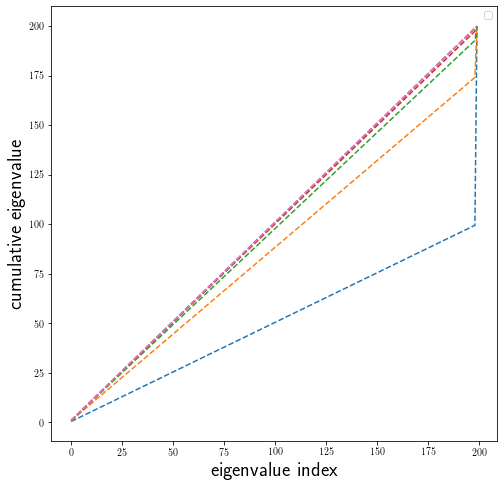
\includegraphics[scale=0.22]{figs/dgn-fra-ecdf-ideal.png}
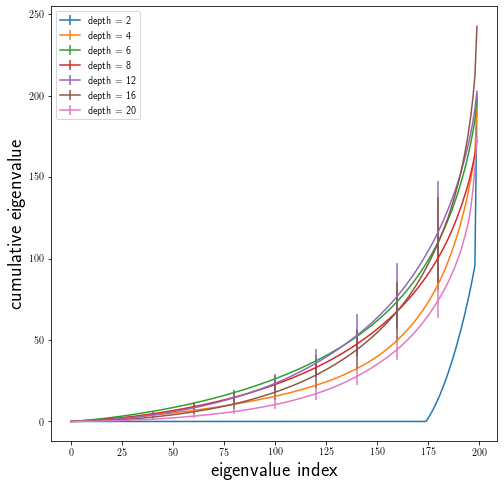
\includegraphics[scale=0.22]{figs/dgn-fra-ecdfbyd-w25.png}
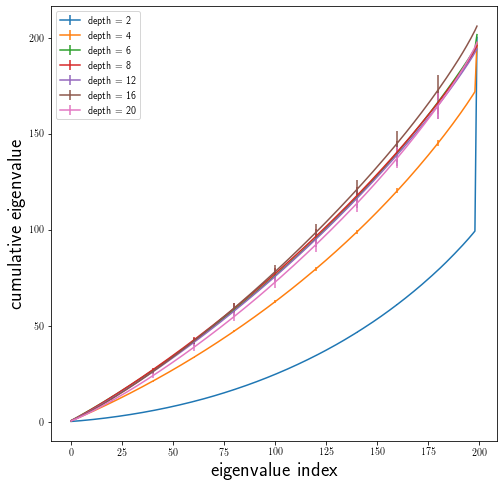
\includegraphics[scale=0.22]{figs/dgn-fra-ecdfbyd-w500.png}
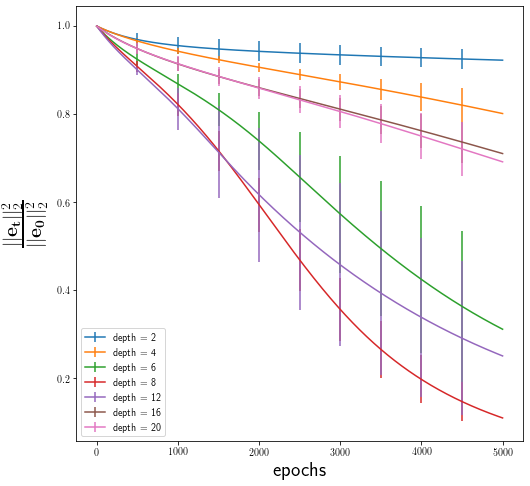
\includegraphics[scale=0.21]{figs/dgn-fra-conv-w25.png}
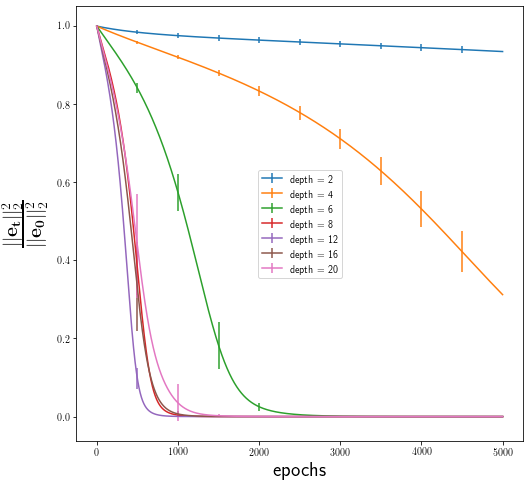
\includegraphics[scale=0.21]{figs/dgn-fra-conv-w500.png}
\caption{Ideal spectrum}
\label{fig:dgn-frg-gram-ecdf}
\end{wrapfigure}
\end{comment}
\begin{comment}
\textbf{A:} In our experiment, we consider DGNs with the following three different gating schemes namely, i) fixed random (FR): for each input example in the dataset, we sample gating values from $Ber(\mu)$ taking values in $\{0,1\}$, and collect it in $\G_0$. DGN with FR gating is useful only for pure memorisation, ii) fixed explicit (FE): gating parameter $\Tg_t=\Tg_0,\forall\, t\geq 0, \Tg_0\neq \Theta_0$, iii) fixed implicit (FI): gating parameter $\Tg_t=\Tg_0,\forall\, t\geq 0, \Tg_0= \Theta_0$. The FI case does not satisfy \Cref{assmp:main}-(i).
\end{comment}
\begin{wrapfigure}{h}{0.20\textwidth}
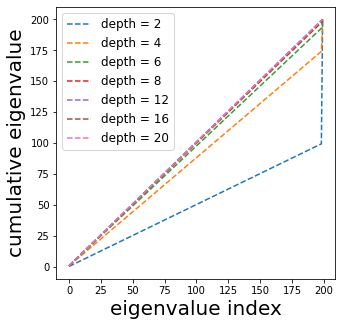
\includegraphics[scale=0.2]{figs/dgn-fra-ecdf-ideal-small.png}
\caption{Ideal spectrum.}
\label{fig:ideal-spectrum}
\end{wrapfigure}
\textbf{Experiment with fixed random gates:} We consider the dataset given by $(x_s,y_s)_{s=1}^n\in \R\times \R$, where $x_s=1,\forall s\in [n]$, and $y_s\sim unif([-1,1])$, $n=200$. For each input example in the dataset, we sample gating values from $Ber(\mu)$ taking values in $\{0,1\}$, and collect it in $\G_0$, which we keep fixed throughout training of the DGN (i.e., $\G_t=\G_0,\,\forall\,t\geq 0$).  Even though the input is the same for all the $n$ examples, via the fixed random gating strategy, we ensure that there is a separate random sub-network for each input example.  In this case, it is easy to check that $\mathbb{E}_{\mu}\left[\lambda_0(s,s)\right]=(\mu w)^{(d-1)},\forall s\in[n]$ and $\mathbb{E}_{\mu}\left[\lambda_0(s,s')\right]=(\mu^2 w)^{(d-1)},\forall s,s'\in[n]$.\WFclear
$\bullet$ \textbf{Spectrum (Ideal):} The input Gram matrix $x^\top x$ is a $n\times n$ matrix with all entries equal to $1$ and its rank is equal to 1, and hence $H_0=\lambda_0$.  For $\sigma=\sqrt{\frac{1}{\mu w}}$, and by further averaging $\mathbb{E}_{\mu}\left[K_0(s,s)/d\right]=1$, and $\mathbb{E}_{\mu}\left[K_0(s,s')/d\right]=\mu^{(d-1)}$. Now, let $\rho_i\geq 0,i \in [n]$ be the eigenvalues of $\frac{\E{K_0}}{d}$, and let $\rho_{\max}$ and $\rho_{\min}$ be the largest and smallest eigenvalues.  One can easily show that $\rho_{\max}=1+(n-1)\mu^{d-1}$ and corresponds to the eigenvector with all entries as $1$, and $\rho_{\min}=(1-\mu^{d-1})$ repeats $(n-1)$ times,  which corresponds to eigenvectors given by $[0, 0, \ldots, \underbrace{1, -1}_{\text{$i$ and $i+1$}}, 0,0,\ldots, 0]^\top \in \R^n$ for $i=1,\ldots,n-1$. Note that as $d\ra\infty$, $\rho_{\max},\rho_{\min}\ra 1$.\\
$\bullet$ \textbf{Spectrum (numerical):} We look at the cumulative eigenvalue (e.c.d.f) obtained by first sorting the eigenvalues in ascending order then looking at their cumulative sum. The ideal behaviour (top plot of \Cref{fig:dgn-frg-gram-ecdf}) as predicted from theory is that for indices $k\in[n-1]$, the e.c.d.f should increase at a linear rate, i.e., the cumulative sum of the first $k$ indices is equal to $k(1-\mu^{d-1})$, and the difference between the last two indices is $1+(n-1)\mu^{d-1}$. In \Cref{fig:dgn-frg-gram-ecdf}, we plot the actual e.c.d.f for various depths $d=2,4,6,8,12,16,20$ and $w=25,500$ a (second and third from top in \Cref{fig:dgn-frg-gram-ecdf}). \hfill\\
$\bullet$ \textbf{Convergence (numerical):} In order to compare how the rate of convergence varies with the depth, we set the step-size $\alpha=\frac{0.1}{\rho_{\max}}$, $w=100$. We use the vanilla SGD-optimiser. Note the$ \frac{1}{\rho_{\max}}$ in the stepsize, ensures that the uniformity of maximum eigenvalue across all the instances, and the convergence should be limited by the smaller eigenvalues. We also look at the convergence rate of the ratio $\frac{\norm{e_t}^2_2}{\norm{e_0}^2_2}$. We notice that for $w=25$, increasing depth till $d=8$ improves the convergence, however increasing beyond $d=8$ worsens the convergence rate. For $w=500$, increasing the depth till $d=12$ improves convergence, and $d=16,20$ are worse than $d=12$.  This matches with the depth phenomena observed in practical DNNs and also matches our theory.
\begin{figure*}[!b]
\resizebox{\textwidth}{!}{
\begin{tabular}{cccc}
%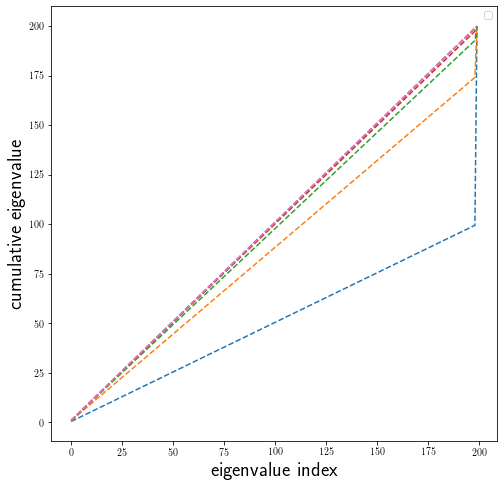
\includegraphics[scale=0.4]{figs/dgn-fra-ecdf-ideal.png}
%&
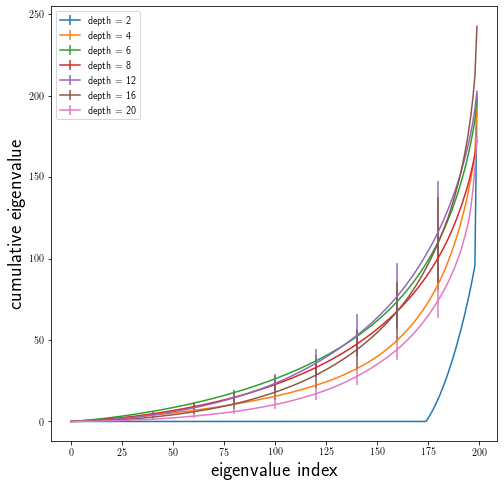
\includegraphics[scale=0.5]{figs/dgn-fra-ecdfbyd-w25.png}
&
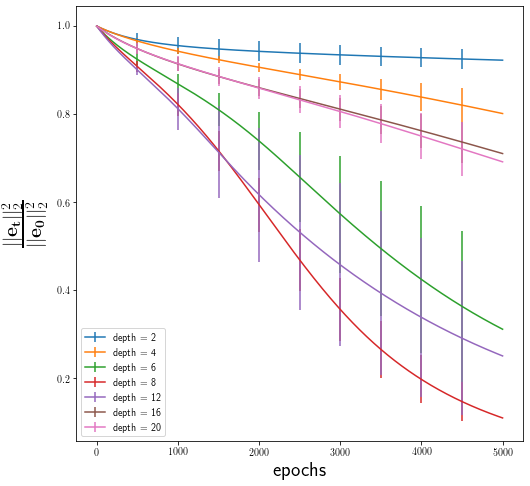
\includegraphics[scale=0.5]{figs/dgn-fra-conv-w25.png}
&
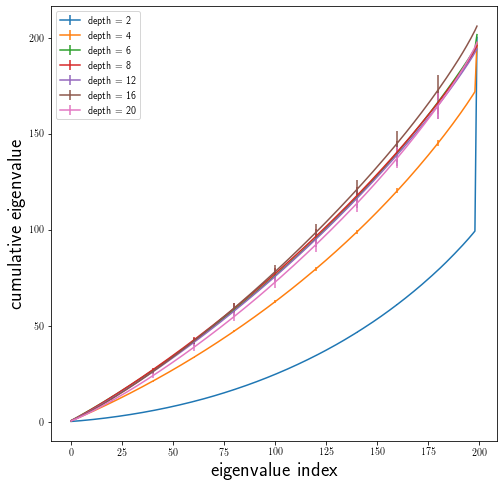
\includegraphics[scale=0.5]{figs/dgn-fra-ecdfbyd-w500.png}
&
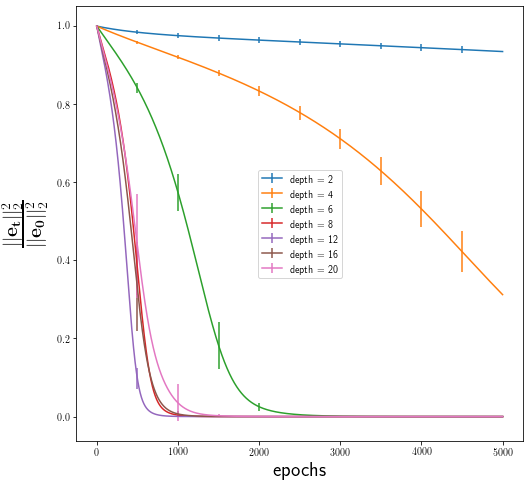
\includegraphics[scale=0.5]{figs/dgn-fra-conv-w500.png}
\end{tabular}
}
\caption{Shows the plots for fixed random gating with $\mu=\frac{1}{2}$ and $\sigma=\sqrt{\frac{2}{w}}$. }
\label{fig:dgn-frg-gram-ecdf}
\end{figure*}


\begin{comment}
\begin{figure}
\resizebox{\textwidth}{!}{
\begin{tabular}{cccc}
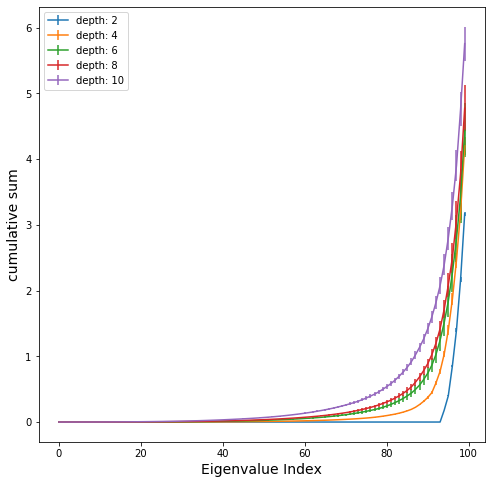
\includegraphics[scale=0.4]{figs/galu-ecdf-d.png}
&
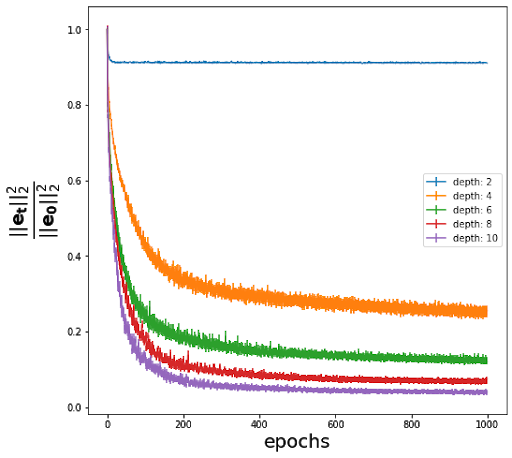
\includegraphics[scale=0.4]{figs/galu-conv-d.png}
&
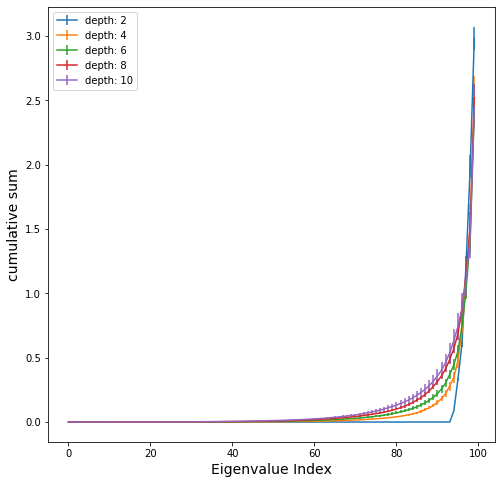
\includegraphics[scale=0.4]{figs/relu-ecdf.png}
&
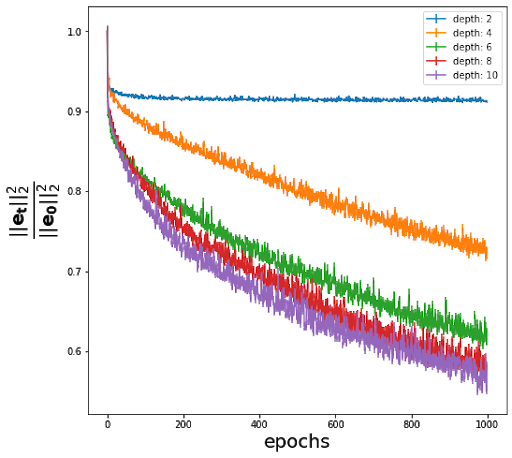
\includegraphics[scale=0.4]{figs/relu-conv.png}
\end{tabular}
}
\caption{The left two plots shows the e.c.d.f and convergence rates for various depth in GaLU networks $w=100$. The third and fourth plot from the left show the e.c.d.f and convergence rates for various depth in ReLU networks $w=100$. The plots are averaged over $5$ runs. }
\label{fig:galu-d}
\end{figure}
\end{comment}

\section{A Note on ConvNets:} 
For input $x\in\R^{d_in}$, consider an architecture with $d_{out}$ channels, and each of which comprises of $d_{conv}$ convolutional layers. Let the convolutional layers perform circular $1$-dimensional convolution with kernel size $d_{ker}<d_{in}$ and unit stride. In the corners, instead of \emph{zero-padding}, in circular convolutional operations, we follow the convention that $\forall l=0,\ldots, d_{conv}-1, k\in[d_{in}], z^{(c)}_{x,t}(l,d_{in}+k)=z^{(c)}_{x,t}(l,k)$, and $z^{(c)}_{x,t}(l,-k)=z^{(c)}_{x,t}(l,d_{in}-k)$, where $z^{(c)}_{x,t}(l)$ is the $d_{in}$ dimensional output of the $l^{th}$ convolutional layer of the channel $c\in[d_{out}]$. The convolutional layers are followed by a \emph{global average-/max-pooling} layer, and arranging all the outputs after pooling we obtain $z_{x,t}(d_{conv}+1)$ to be the $d_{out}$-dimensional output, which is then followed by fully connected layers. Owing to the inherent circular (cylindrical) symmetry at all the convolutional layers, the $d_{out}$ dimensional feature produced after the pooling layers is invariant to circular shifts in the input.

\section{Proofs}
\textbf{Statement of \Cref{lm:npk}}
 Let $x=(x_s,s\in [n])\in\R^{d_{in}\times n}$ be the data matrix and let the neural path kernel matrix be defined as $H_t\stackrel{def}=\Phi^\top_t\Phi_t$. It follows that $H_t= (x^\top x)\odot(\lambda_t)$. 
\begin{proof}
\begin{align*}
\phi^\top_{x_s,t}\phi_{x_s',t}&=\sum_{p\in[P]}x(\I_0(p),s)A_t(x_s,p) x(\I_0(p),s')A_t(x_{s'},p)\\
&=\sum_{i=1}^{d_{in}}\sum_{p\rsa i}x(i,s)A_t(x_s,p) x(i,s')A_t(x_{s'},p)\\
&=\sum_{i=1}^{d_{in}}x_s(i)x_{s'}(i)\sum_{p\rsa i} A_t(x_s,p)A_t(x_{s'},p)\\
&=(x^\top_s x_{s'})\lambda_t(s,s')
\end{align*}
\end{proof}

\textbf{Statement of \Cref{lm:disentangle}}
Under \Cref{assmp:main}, for paths $p,p'\in \P, p\neq p'$, we have  i) $\E{\ip{\varphi_{p,0}, \varphi_{p',0}}}= 0$ and ii)${\ip{\varphi_{p,0}, \varphi_{p,0}}}= d\sigma^{2(d-1)}$.
\begin{proof}
\begin{align*}
\ip{\varphi_{p,t}, \varphi_{p',t}}= \sum_{m=1}^{d_{net}} \varphi_{p,t}(m)\varphi_{p',t}(m)
\end{align*}
Let the $d_{net}$ weights be enumerable as $\theta(1),\ldots,\theta(d_{net})$, and let $\theta(m),m\in[d_{net}]$ be any weight such that $p\rsa \theta(m)$, and w.l.o.g let $\theta(m)$ belong to layer $l'(m)\in[d]$. 
If either $p\bcancel{\rsa}\theta(m)$ or $p'\bcancel{\rsa}\theta(m)$, then it follows that $\varphi_{p,t}(m)\varphi_{p',t}(m)=0$. In the case when $p,p'\rsa\theta(m)$, we have
\begin{align*}
&\E{\varphi_{0,p}(m)\varphi_{0,p'}(m)}\\
&=\E{\underset{l\neq l'(m)}{\underset{l=1}{\overset{d}{\Pi}}} \Bigg(\Tb_0(l,\I_{l-1}(p),\I_l(p))\Tb_0(l,\I_{l-1}(p'),\I_l(p')) \Bigg)}\\
&=\underset{l\neq l'(m)}{\underset{l=1}{\overset{d}{\Pi}}}\E{\Tb_0(l,\I_{l-1}(p),\I_l(p))\Tb_0(l,\I_{l-1}(p'),\I_l(p'))}
\end{align*}
where the $\E{\cdot}$ moved inside the product because at initialisation the weights (of different layers) are independent of each other.
Since $p\neq p'$, in one of the layers $\tilde{l}\in[d-1],\tilde{l}\neq l'(m)$ they do not pass through the same weight, i.e., $\Tb_0(\tilde{l},\I_{\tilde{l}-1}(p),\I_{\tilde{l}}(p))$ and $\Tb_0(\tilde{l},\I_{\tilde{l}-1}(p'),\I_{\tilde{l})}(p')$ are distinct weights. Using this fact
\begin{align*}
&\E{\varphi_{0,p}(m)\varphi_{0,p'}(m)}\\
&=\underset{l\neq l',\tilde{l}}{\underset{l=1}{\overset{d}{\Pi}}}\E{\Tb_0(l,\I_{l-1}(p),\I_l(p))\Tb_0(l,\I_{l-1}(p'),\I_l(p'))}\E{\Tb_0(\tilde{l},\I_{\tilde{l}-1}(p),\I_{\tilde{l}}(p))}\E{\Tb_0(\tilde{l},\I_{\tilde{l}-1}(p'),\I_{\tilde{l}}(p')}\\\\
&=0
\end{align*}

The proof of (ii) is complete by noting that $\sum_{m=1}^{d_{net}} \varphi_{p,t}(m)\varphi_{p,t}(m)$ has $d$ non-zero terms for a single path $p$ and at initialisation we have 
\begin{align*}
&{\varphi_{0,p}(m)\varphi_{0,p}(m)}\\
&={\underset{l\neq l'}{\underset{l=1}{\overset{d}{\Pi}}} \Tb^2_0(l,\I_{l-1}(p),\I_l(p))}\\
&=\sigma^{2(d-1)}
\end{align*}
\end{proof}

\textbf{Statement of \Cref{th:exp}}
Under \Cref{assmp:main}, we have $\E{K_0}=d\sigma^{2(d-1)}(x^\top x) \odot (\lambda_0)$.

\begin{proof} Let $\varphi_t=\left[\varphi_{p,t},p\in[P]\right]\in\R^{d_{net}\times P}$ be the VTF matrix at time $t$, then if follows that the NTK (Gram) matrix is  $K_t=\Psi^\top_t\Psi_t=\Phi^\top_t\varphi_t\varphi^\top_t\Phi_t$. Now, taking expectation we have $\E{K_0}=\E{\Phi^\top_t\varphi_t\varphi^\top_t\Phi_t}$, and using \Cref{assmp:main}-(i), one can pull out the $\Phi_t$ terms outside of the expectation, i,e., $\E{K_0}=\Phi^\top_t\E{\varphi_t\varphi^\top_t}\Phi_t$, and using \Cref{assmp:main}-(ii), we can show that $\E{\varphi_t\varphi^\top_t}=d\sigma^{2(d-1)}I$. The statement of \Cref{th:exp} follows by using \Cref{lm:npk}.
\end{proof}


\textbf{Statement of \Cref{th:var}}
Under \Cref{assmp:main} and the condition that ${4d}/{w^2}<1$, it follows that\hfill\\
$Var\left[K_0\right]\leq O\left(d^2_{in}\sigma^{4(d-1)}\max\{d^2w^{2(d-2)+1}, d^3w^{2(d-2)}\}\right)$.
\begin{proof}
The idea is that we expand  $Var\left[K_0(s,s')\right]=\E{K_0(s,s')^2} -\E{K_0(s,s')}^2$ and identify the the terms which cancel due to subtraction and then bound the rest of the terms.% Further, in what follows, we will assume $d_{in}=1$ without loss of generality.
 Let $\theta(m)$ belong to layer $l'(m)$, then 
\begin{align}\label{eq:kexpect}
&\E{K_0(s,s')}\nn\\
&=\sum_{m=1}^{d_{net}}\E{\left(\sum_{p_1 \in[P]}x(\I_0(p_1),s)A_0(s,p_1)\frac{\partial v_0(p_1)}{\partial \theta(m)}\right)\left(\sum_{p_2\in[P]}x(\I_0(p_2),s)A_0(s',p_2)\frac{\partial v_0(p_2)}{\partial \theta(m)}\right)}\nn\\
&=\sum_{m=1}^{d_{net}}\E{\sum_{p_1,p_2\in[P]}x(\I_0(p_1),s)A_0(s,p_1)\frac{\partial v_0(p_1)}{\partial \theta(m)}x(\I_0(p_2),s')A_0(s',p_2)\frac{\partial v_0(p_2)}{\partial \theta(m)}}\nn\\
&\stackrel{(a)}=\sum_{m=1}^{d_{net}}\underset{p_1,p_2\rsa\theta(m)}{\sum_{p_1,p_2\in[P]}}x(\I_0(p_1),s)A_0(s,p_1)x(\I_0(p_2),s')A_0(s',p_2) \E{\underset{l\neq l'(m)}{\underset{l=1}{\overset{d-1}{\Pi}}} \Tb_0(l,\I_{l-1}(p_1),\I_{l}(p_1)) \Tb_0(l,\I_{l-1}(p_2),\I_{l}(p_2))}\nn\\
&\stackrel{(b)}=\sum_{m=1}^{d_{net}}\underset{p_1,p_2\rsa\theta(m)}{\sum_{p_1,p_2\in[P]}}x(\I_0(p_1),s)A_0(s,p_1)x(\I_0(p_2),s')A_0(s',p_2) \underset{l\neq l'(m)}{\underset{l=1}{\overset{d-1}{\Pi}}} \E{\Tb_0(l,\I_{l-1}(p_1),\I_{l}(p_1)) \Tb_0(l,\I_{l-1}(p_2),\I_{l}(p_2))}
\end{align}
where $(a)$ follows from the fact that for $p\bcancel{\rsa}\theta(m)$, $\frac{\partial v_0(p)}{\partial \theta(m)}=0$, and $(b)$ follows from the fact that at initialisation the layer weights are independent of each other. Note that the right hand side of \eqref{eq:kexpect} only terms with $p_1=p_2$ will survive the expectation.

In the following expression in \eqref{eq:kexpectsquare}, note that only terms of the form $p_1=p_2$ and $p_3=p_4$ are non-zero.
\begin{align}\label{eq:kexpectsquare}
&\E{K_0(s,s')}^2=\nn\\
&\left(\sum_{m=1}^{d_{net}}\underset{p_1,p_2\rsa\theta(m)}{\sum_{p_1,p_2\in[P]}}x(\I_0(p_1),s)A_0(s,p_1)x(\I_0(p_2),s')A_0(s',p_2) \underset{l\neq l'(m)}{\underset{l=1}{\overset{d-1}{\Pi}}} \E{\Tb_0(l,\I_{l-1}(p_1),\I_{l}(p_1)) \Tb_0(l,\I_{l-1}(p_2),\I_{l}(p_2))}\right)\nn\\
&\left(\sum_{m'=1}^{d_{net}}\underset{p_3,p_4\rsa\theta(m')}{\sum_{p_3,p_4\in[P]}}x(\I_0(p_3),s)A_0(s,p_3)x(\I_0(p_4),s')A_0(s',p_4) \underset{l\neq l'(m')}{\underset{l=1}{\overset{d-1}{\Pi}}} \E{\Tb_0(l,\I_{l-1}(p_3),\I_{l}(p_3)) \Tb_0(l,\I_{l-1}(p_4),\I_{l}(p_4))}\right)\nn\\
&=\nn\\
&\sum_{m,m'=1}^{d_{net}}\underset{p_3,p_4\rsa\theta(m')}{\underset{p_1,p_2\rsa\theta(m)}{\sum_{p_1,p_2,p_3,p_4\in[P]}}}\Bigg[\bigg(x(\I_0(p_1),s)A_0(s,p_1)x(\I_0(p_2),s')A_0(s',p_2)x(\I_0(p_3),s)A_0(s,p_3)x(\I_0(p_4),s')A_0(s',p_4)\bigg)\nn\\
&\bigg( \underset{l\neq l'(m)} {\underset{l\neq l'(m')}{\underset{l=1}{\overset{d-1}{\Pi}}}} \E{\Tb_0(l,\I_{l-1}(p_1),\I_{l}(p_1)) \Tb_0(l,\I_{l-1}(p_2),\I_{l}(p_2))}\E{\Tb_0(l,\I_{l-1}(p_3),\I_{l}(p_3)) \Tb_0(l,\I_{l-1}(p_4),\I_{l}(p_4))} \bigg)\nn\\
&\bigg( \E{\Tb_0(l,\I_{l'(m')-1}(p_1),\I_{l'(m')}(p_1)) \Tb_0(l,\I_{l'(m')-1}(p_2),\I_{l'(m')}(p_2))}\bigg)\nn\\
&\bigg(\E{\Tb_0(l,\I_{l'(m)-1}(p_3),\I_{l'(m)}(p_3)) \Tb_0(l,\I_{l'(m)-1}(p_4),\I_{l'(m)}(p_4))} \bigg)\Bigg]\nn\\
\end{align}

In the expression in \eqref{eq:ksquareexpect}, paths $p_1,p_2,p_3,p_4$ do not have constraints, and can be distinct.
\begin{align}\label{eq:ksquareexpect}
&\E{K^2_0(s,s')}=\nn\\
&\sum_{m,m'=1}^{d_{net}}\underset{p_3,p_4\rsa\theta(m')}{\underset{p_1,p_2\rsa\theta(m)}{\sum_{p_1,p_2,p_3,p_4\in[P]}}}\Bigg[\bigg(x(\I_0(p_1),s)A_0(s,p_1)x(\I_0(p_2),s')A_0(s',p_2)x(\I_0(p_3),s)A_0(s,p_3)x(\I_0(p_4),s')A_0(s',p_4)\bigg)\nn\\
&\bigg( \underset{l\neq l'(m)} {\underset{l\neq l'(m')}{\underset{l=1}{\overset{d-1}{\Pi}}}} \E{\Tb_0(l,\I_{l-1}(p_1),\I_{l}(p_1)) \Tb_0(l,\I_{l-1}(p_2),\I_{l}(p_2))\Tb_0(l,\I_{l-1}(p_3),\I_{l}(p_3)) \Tb_0(l,\I_{l-1}(p_4),\I_{l}(p_4))} \bigg)\nn\\
&\bigg( \E{\Tb_0(l,\I_{l'(m')-1}(p_1),\I_{l'(m')}(p_1)) \Tb_0(l,\I_{l'(m')-1}(p_2),\I_{l'(m')}(p_2))}\bigg)\nn\\
&\bigg(\E{\Tb_0(l,\I_{l'(m)-1}(p_3),\I_{l'(m)}(p_3)) \Tb_0(l,\I_{l'(m)-1}(p_4),\I_{l'(m)}(p_4))} \bigg)\Bigg]\nn\\
\end{align}

We now state the following facts/observations.

$\bullet$ \textbf{Fact 1:} Any term that survives the expectation (i.e., does not become $0$) and participates in \eqref{eq:ksquareexpect} is of the form $\sigma^{4(d-1)}\big(x(\I_0(p_1),s)A_0(s,p_1)x(\I_0(p_2),s')A_0(s',p_2)x(\I_0(p_3),s)A_0(s,p_3)x(\I_0(p_4),s')A_0(s',p_4)\big)$, where $p_1,p_2,p_3,p_4$ are free variables. Any term that survives the expectation (i.e., does not become $0$) and participates in participates in \eqref{eq:kexpectsquare} is of the form $\sigma^{4(d-1)}\big(x(\I_0(p_1),s)A_0(s,p_1)x(\I_0(p_2),s')A_0(s',p_2)x(\I_0(p_3),s)A_0(s,p_3)x(\I_0(p_4),s')A_0(s',p_4)\big)$, where $p_1=p_2,p_3=p_4$.

$\bullet$ \textbf{Fact 2:} The number of paths through a particular weight $\theta(m)$ in one of the middle layers is $d_{in}w^{d-3}$, and the number of paths through a particular weight $\theta(m)$ in either the first or the last layer is $d_{in}w^{d-2}$ .

$\bullet$ \textbf{Fact 3:} Let $\P'$ be an arbitrary set of paths constrained to pass through some set of weights. Let $\P''$ be the set of paths obtained by adding an additional constraint that the paths also should pass through a particular weight say $\theta(m)$. Now, if $\theta(m)$ belongs to :

$1.$ a middle layer, then $|\P''|=\frac{|\P'|}{w^2}$.

$2.$ the first layer or the last layer, then $|\P''|=\frac{|\P'|}{w}$.

$\bullet$ \textbf{Fact 4:} For any $p_1,p_2,p_3,p_4$ combination that survives the expectation in \eqref{eq:ksquareexpect} can be written as 

\begin{align*}
&\bigg( \underset{l\neq l'(m)} {\underset{l\neq l'(m')}{\underset{l=1}{\overset{d-1}{\Pi}}}} \E{\Tb_0(l,\I_{l-1}(p_1),\I_{l}(p_1)) \Tb_0(l,\I_{l-1}(p_2),\I_{l}(p_2))\Tb_0(l,\I_{l-1}(p_3),\I_{l}(p_3)) \Tb_0(l,\I_{l-1}(p_4),\I_{l}(p_4))} \bigg)\nn\\
&\bigg( \E{\Tb_0(l,\I_{l'(m')-1}(p_1),\I_{l'(m')}(p_1)) \Tb_0(l,\I_{l'(m')-1}(p_2),\I_{l'(m')}(p_2))}\bigg)\nn\\
&\bigg(\E{\Tb_0(l,\I_{l'(m)-1}(p_3),\I_{l'(m)}(p_3)) \Tb_0(l,\I_{l'(m)-1}(p_4),\I_{l'(m)}(p_4))} \bigg)\Bigg]\nn\\
&=\\
&\bigg( \underset{l\neq l'(m)} {\underset{l\neq l'(m')}{\underset{l=1}{\overset{d-1}{\Pi}}}} \Tb^2_0(l,\I_{l-1}(\rho_a),\I_{l}(\rho_a)) \Tb^2_0(l,\I_{l-1}(\rho_b),\I_{l}(\rho_b)) \bigg)\nn\\
&\bigg( \Tb^2_0(l,\I_{l'(m')-1}(\rho_a),\I_{l'(m')}(\rho_a))\bigg)\nn\\
&\bigg({\Tb^2_0(l,\I_{l'(m)-1}(\rho_b),\I_{l'(m)}(\rho_b))} \bigg),
\end{align*}

where $\rho_a\rsa \theta(m)$ and $\rho_b\rsa \theta(m')$ are what we call as \emph{base} (case) paths. 


$\bullet$ \textbf{Fact 5:} For any given base paths $\rho_a$ and $\rho_b$ there could be multiple assignments possible for $p_1,p_2,p_3,p_4$.

$\bullet$ \textbf{Fact 6:}  Terms in \eqref{eq:ksquareexpect}, wherein, the base case is generated as $p_1=p_2=\rho_a$ and $p_3=p_4=\rho_b$ (or $p_1=p_2=\rho_b$ and $p_3=p_4=\rho_a$), get cancelled with the corresponding terms in \eqref{eq:kexpectsquare}.

$\bullet$ \textbf{Fact 7:}  When the bases paths $\rho_a$ and $\rho_b$ do not intersect (i.e., do not pass through the same weight in any one of the layers), the only possible assignment is $p_1=p_2=\rho_a$ and $p_3=p_4=\rho_b$ (or $p_1=p_2=\rho_b$ and $p_3=p_4=\rho_a$), and such terms are common in \eqref{eq:ksquareexpect} and \eqref{eq:kexpectsquare}, and hence do not show up in the variance term.


$\bullet$ \textbf{Fact 7:} Let base paths $\rho_a$ and $\rho_b$ intersect/cross at layer $l_1, \ldots, l_k, k \in [d-1]$, and let $\rho_a=(\rho_a(1),\ldots,\rho_a(k+1))$ where $\rho_a(1)$ is a sub-path string from layer $1$ to $l_1$, and $\rho_a(2)$ is the sub-path string from layer $l_1+1$ to $l_2$ and so on, and $\rho_a(k+1)$ is the sub-path string from layer $l_k+1$ to the output node. Then the set of paths that can occur in $\E{K_0(s,s')^2}$ are of the form:
\begin{enumerate}
\item $p_1=p_2=\rho_a, p_3=p_4=\rho_b$ (or $p_1=p_2=\rho_b, p_3=p_4=\rho_a$) which get cancelled in the $\E{K_0(s,s')}^2$ term.
\item $p_1=\rho_a$, $p_3=\rho_b$, $p_2=(\rho_b(1),\rho_a(2),\rho_a(3),\ldots,\rho_a(k+1))$, $p_4=(\rho_a(1),\rho_b(2),\rho_b(3),\ldots,\rho_b(k+1))$, which are obtained by splicing the base paths in various combinations. Note that for such spliced paths $p_1\neq p_2$ and $p_3\neq p_4$ and hence do not occur in the expression for $\E{K_0(s,s')}^2$ in \eqref{eq:kexpectsquare}.
\end{enumerate}


$\bullet$ \textbf{Fact 8:} For $k$ crossings of the base paths there are $4^{k+1}$ splicings possible, and those many terms are extra in the $\E{K_0(s,s')^2}$ expression in \eqref{eq:ksquareexpect}, when compared to the $\E{K_0(s,s')}^2$ expression. We now enumerate cases of possible crossings, and reason out the magnitude of their contribution to the variance term using the \textbf{Fact 1} to \textbf{Fact 8}.


\textbf{Case $1$} $k=1$ crossing in either first or last layer. There are $2w$ weights in the first and the last layer, and the number of base path combinations is $w^{d-2}\times w^{d-2}$, and for each of these cases, $m,m'$ could take $O(d^2)$ possible values. And the multiplication of the weights themselves contribute to $\sigma^{4(d-1)}$. Putting them together we have
\begin{align*}
d^2_{in}\sigma^{4(d-1)}\times (2w)\times d^2\times (w^{d-2}\times w^{d-2})\times 4^2 = 32d^2_{in}\sigma^{4(d-1)}d^2 w^{2(d-2)+1}
\end{align*}

\textbf{Case $2$} $k=1$ crossing in one of the middle layers. There are $w^2(d-2)$ weights in the first and the last layer, and the number of base path combinations is $w^{d-3}\times w^{d-3}$, and for each of these cases, $m,m'$ could take $O(d^2)$ possible values. And the multiplication of the weights themselves contribute to $\sigma^{4(d-1)}$. Putting them together we have
\begin{align*}
d^2_{in}\sigma^{4(d-1)}\times w^2(d-2)\times d^2\times (w^{d-3}\times w^{d-3})\times 4^2\leq 16d^2_{in}\sigma^{4(d-1)} d^3 w^{2(d-3)}
\end{align*}

\textbf{Case $3$} $k=2$ crossings one in the first layer and other in the last layer. This case can be covered using Case $1$ and then further restricting that the base paths should also in the other layer. So, we have
\begin{align*}
32d^2_{in}\sigma^{4(d-1)}d^2 w^{2(d-2)+1} \times \underbrace{w}_{\text{possible weights in other layer}} \times \underbrace{w^{-1}\times w^{-1}}_{\text{reduction in paths due to additional restriction}} \times 4 = (32d^2_{in}\sigma^{4(d-1)}d^2 w^{2(d-2)+1})\times (4w^{-1}),
\end{align*}
where the $4$ is for the $4$ extra possible ways of splicing the base paths.

\textbf{Case $4$} $k=2$ crossings first one in the first layer or the last layer, and the second one in the middle layer. This can be obtained by looking at the Case $1$ and then adding the further restriction that the base paths should cross each other in the middle layer. 
\begin{align*}
32d^2_{in}\sigma^{4(d-1)}d^2 w^{2(d-2)+1}\times w^2(d-2) \times (w^{-2}w^{-2}) \times 4= (32d^2_{in}\sigma^{4(d-1)}d^2 w^{2(d-2)+1} )\times (4dw^{-2}) 
\end{align*}

\textbf{Case $5$} $k=2$ crossings in the middle layer. This can be obtained by taking Case $2$ and then adding the further restriction that the base paths should cross each other in the middle layer. 
\begin{align*}
16d^2_{in}\sigma^{4(d-1)} d^3 w^{2(d-3)}\times w^2(d-2) w^{-2}w^{-2}\times 4\leq (16d^2_{in}\sigma^{4(d-1)} d^3 w^{2(d-3)}) \times (4dw^{-2})
\end{align*}


\textbf{Case $6$} $k=3$ crossings first one in the first layer or the last layer, and the other two in the middle layers. This can be obtained by considering Case $4$ and then adding the further restriction that the base paths should cross each other in the middle layer. 
\begin{align*}
(32d^2_{in}\sigma^{4(d-1)}d^2 w^{2(d-2)+1} )\times (4dw^{-2}) \times (4dw^{-2}) 
\end{align*}

\textbf{Case $7$} $k=3$ crossings first two in the first and last layers and the third one in the middle layers. This can be obtained by considering Case $3$ and then adding the further restriction that the base paths should cross each other in the middle layer. 

\begin{align*}
(32d^2_{in}\sigma^{4(d-1)}d^2 w^{2(d-2)+1})\times (4w^{-1})\times (4dw^{-2}) 
\end{align*}

\textbf{Case $8$} $k=3$ crossings in the middle layer. This can be obtained by considering Case $5$ and then adding the further restriction that the base paths should cross each other in the middle layer. 
\begin{align*}
 (16d^2_{in}\sigma^{4(d-1)} d^3 w^{2(d-3)}) \times (4dw^{-2})\times (4dw^{-2}) 
\end{align*}


The cases can be extended in a similar way, increasing the number of crossings.  Now, assuming $\frac{4d}{w^2}<1$, the bounds in the various terms can be lumped together as below:

$\bullet$ We can add the bounds for Case $1$, Case $4$, Case $6$ and other cases obtained by adding more crossings (one at a time) in the middle layer to Case $6$. This gives rise to a term which is upper bounded by 
\begin{align*}
d^2_{in}\sigma^{4(d-1)}d^2w^{2(d-2)+1}\left(\frac{1}{1-4dw^{-2}}\right)
\end{align*}

$\bullet$ We can add the bounds for Case $3$, Case $7$ and other cases obtained by adding more crossings (one at a time) in the middle layer to Case $6$. This gives rise to a term which is upper bounded by 
\begin{align*}
d^2_{in}\sigma^{4(d-1)}d^3w^{2(d-2)} \left(\frac{1}{1-4dw^{-2}}\right)
\end{align*}



$\bullet$ We can add the bounds for Case $2$, Case $5$, Case $8$ and other cases obtained by adding more crossings (one at a time) in the middle layer to Case $6$. This gives rise to a term which is upper bounded by 
\begin{align*}
d^2_{in}\sigma^{4(d-1)}d^2w^{2(d-2)} \left(\frac{1}{1-4dw^{-2}}\right)
\end{align*}

Putting together we have the variance to be bounded by 
\begin{align*}
Cd^2_{in}\sigma^{4(d-1)}\max\{d^2w^{2(d-2)+1}, d^3w^{2(d-2)}\},
\end{align*}
for some constant $C>0$.
\end{proof}
